\section*{Question 1}
Meet, from left to right, Joe, William, Jack and Averell, villains of our childhood that go by the name of the Dalton brothers. These inseparable brothers have a special rule among themselves. They always stand in order of their height.

Write a program \texttt{TheDaltons.java} that takes names of the brothers as command-line arguments and prints \texttt{false} unless the order in which arguments are given follows \textit{The Dalton Rule}.

Example:\\
\texttt{\% java TheDaltons Joe William Jack Averell > true}\\
\texttt{\% java TheDaltons Averell Jack William Joe > true}\\
\texttt{\% java TheDaltons Averell William Joe Jack > false}

\begin{figure}[H]\centering
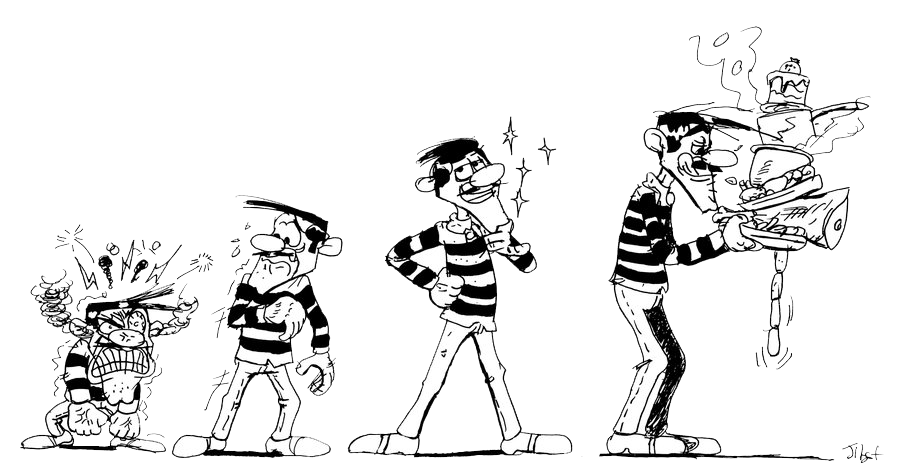
\includegraphics{\topDirectory/template/images/daltons.png}
\caption{The Dalton Brothers}
\end{figure}

\section*{Question 2}

Matthew and John are playing backgammon and they hate rolling the two dice each turn, over and over again.

\begin{enumerate}
\item Write a program \texttt{Dice1.java} that gives two random integer numbers from one to six each time it is executed.
\item Upgrade your program to \texttt{Dice2.java} such that it takes an integer number as command-line argument and generates two random integer values in the range of one to given integer number.
\end{enumerate}
